% main.tex -- draft manuscript.  Build: see Makefile (latex+bibtex+dvips with the EPS figures, or
% pdflatex with the PDF copies of the same figures).  Every table is \input from tables/*.tex,
% which make_tables.py writes from results/*.json; figures come from make_eps.py.
\documentclass[pra,twocolumn,superscriptaddress,longbibliography]{revtex4-2}
\usepackage{amsmath,amssymb,bm}
\usepackage{graphicx}       % latex -> figures/*.eps,  pdflatex -> figures/*.pdf
\usepackage{xcolor}
\usepackage[colorlinks=true,linkcolor=blue,citecolor=blue,urlcolor=blue]{hyperref}

% ---- authorship switch ---------------------------------------------------------------------
% \aiauthorfalse : F. C. Moreira sole author; the AI's part is stated under "Use of AI" in the
%                  acknowledgments (arXiv and APS do not accept AI systems as authors).
% \aiauthortrue  : would list the AI as a second author (see PLAN.md, Sec. 6).
\newif\ifaiauthor
\aiauthorfalse

% ---- review aids (set \showtodosfalse for submission) -------------------------------------
\newif\ifshowtodos
\showtodostrue
\newcommand{\todo}[1]{\ifshowtodos\textcolor{red}{[TODO: #1]}\fi}

\newcommand{\PT}{\mathcal{PT}}
\newcommand{\chit}{\chi^{(2)}}
\newcommand{\Img}{\mathrm{Im}\,}
\newcommand{\Rea}{\mathrm{Re}\,}
\newcommand{\dd}{\mathrm{d}}

\begin{document}

\title{Gap solitons in a $\chit$ waveguide with a $\PT$-symmetric lattice revisited:\\
edge shooting, symmetric Newton continuation, and spectral stability}

\author{F. C. Moreira}
\affiliation{Universidade Federal de Alagoas, Macei\'o--AL, Brazil \todo{confirm current affiliation}}
\ifaiauthor
\author{Claude Opus 5.5}
\affiliation{Anthropic (AI system); numerical code, computations and first draft produced in Claude Code}
\fi

\date{\today}

\begin{abstract}
We revisit the model of fundamental-frequency (FF) and second-harmonic (SH) waves coupled by the
quadratic ($\chit$) nonlinearity in a periodic potential whose FF part carries balanced gain and
loss, $V_1\cos 2\xi + i\alpha\sin 2\xi$ [Phys.\ Rev.\ A \textbf{87}, 013832 (2013)]. The
numerical chain was rebuilt from scratch and validated piece by piece. It consists of the Floquet
band structure, edge shooting from the decaying Floquet tails with an adaptive
Runge--Kutta--Fehlberg integrator, cubic-spline transfer to a Newton--Raphson solver on a
$\PT$-symmetric half domain, continuation in $\alpha$ and in the propagation constant $b$, linear
stability with a complex absorbing layer, and split-step Fourier propagation. The band structure,
the matching of the band edges and the soliton families of the original work are reproduced once a
sign convention is corrected ($b\to-b$ in the printed stationary equations). Three results differ
from the original analysis. The fundamental soliton of the third finite gap is centred at the
lattice minimum. The conservative ($\alpha=0$) third-gap family, drawn as stable, has an
oscillatory instability with growth rate up to $0.087$, which direct propagation confirms; the gain
and loss weaken it by more than an order of magnitude but do not remove it. Finally,
instabilities with rates of order $10^{-3}$ occur inside parameter windows reported as stable, and
seeded propagation reproduces their rates to within 5\%. Code, data and every figure are provided
for reproduction.
\end{abstract}

\maketitle

% =============================================================================================
\section{Introduction}
Parity--time ($\PT$) symmetric systems, with spatially separated and mutually balanced gain and
loss, can have a purely real spectrum below a threshold of the gain--loss strength
\cite{Bender1998,Bender2007}. Optics turned the idea into experiments \cite{Ruter2010}. Periodic
$\PT$ potentials and the solitons they support became a central topic
\cite{Makris2008,Musslimani2008,Nixon2012,Abdullaev2011,Zezyulin2012,Konotop2016,ElGanainy2018}.
In quadratic media the soliton is a bound state of the FF and SH waves
\cite{Etrich2000,Buryak2002}. Combining $\chit$ nonlinearity with $\PT$ potentials, a localized
potential was considered first \cite{Moreira2012}, and periodic potentials in
Ref.~\cite{MKM2013}.

Here we re-derive the soliton families and their stability for the periodic model of
Ref.~\cite{MKM2013}. The numerical chain follows the algorithms of the thesis
\cite{MoreiraThesis}: edge shooting with interstep refinement, then cubic splines feeding a
Newton--Raphson solver, then split-step propagation. Each step was re-implemented independently,
in a few thousand lines of plain Python and NumPy, and each building block is validated against a
known answer (Sec.~\ref{sec:validation}). The aim is to provide a reproducible reference
implementation, and to separate the results that survive the stricter numerical tests from those
that do not.

% =============================================================================================
\section{Model}\label{sec:model}
We write the evolution equations as
\begin{align}
i\partial_\zeta u_1 &= -\partial_\xi^2 u_1 - U_1(\xi)\,u_1 - 2u_1^{*}u_2, \label{eq:u1}\\
i\partial_\zeta u_2 &= -\tfrac12\partial_\xi^2 u_2 - U_2(\xi)\,u_2 - u_1^{2}, \label{eq:u2}
\end{align}
with $U_1 = V_1\cos 2\xi + i\alpha\sin 2\xi$ and $U_2 = 2(V_2\cos 2\xi + q)$. Here $q$ is the
phase mismatch. Stationary states $u_l = w_l(\xi)e^{ilb\zeta}$ obey
\begin{align}
w_1'' + \left[V_1\cos 2\xi + i\alpha\sin 2\xi - b\right]w_1 + 2w_1^{*}w_2 &= 0, \label{eq:w1}\\
\tfrac12 w_2'' + 2\left[V_2\cos 2\xi + q - b\right]w_2 + w_1^{2} &= 0. \label{eq:w2}
\end{align}
The power is $P = P_1 + P_2$ with $P_l = l\int|w_l|^2\dd\xi$, and the currents are
$j_l = \Img(w_l^{*}w_l')$.

The $\PT$ symmetry $U_1(-\xi) = U_1^{*}(\xi)$ admits solutions with $w_l(-\xi) = w_l^{*}(\xi)$:
$\Rea w_l$ is even and $\Img w_l$ is odd. The lattice $V_l\cos2\xi$ has two symmetry points per period: $\xi=0$, a lattice maximum, and
$\xi=\pi/2$, a lattice minimum. In Schr\"odinger form the effective potential is
$-V_l\cos2\xi$, so these are its minimum and maximum, respectively. Solitons centred at $\xi_0$ are
obtained by replacing $\xi\to\xi+\xi_0$ in the potentials, with $\xi$ measured from the centre.

\paragraph*{Relation to the printed equations.}
Equations~(\ref{eq:w1})--(\ref{eq:w2}) are the stationary equations of Ref.~\cite{MKM2013} with
$b\to-b$. With the printed sign, the top edge of the SH Mathieu band lies at $b=-0.378$ and the
semi-infinite gap extends to $b\to-\infty$. The numbers in the figures of Ref.~\cite{MKM2013},
namely $b_{2+}^{(0)} = 0.3784$, $q_+^{(0,0)} = -0.316$, the third-gap coalescence at
$b\approx-1.29$ and the semi-infinite gap at $b > 0.378$, are reproduced only after $b\to-b$.
Equations~(\ref{eq:u1})--(\ref{eq:u2}) are the printed evolution equations with $\zeta\to-\zeta$.
This is equivalent to the mirror image $\xi\to-\xi$ of the gain--loss pattern, so it changes
neither existence nor stability. The currents change sign, which we observe.

% =============================================================================================
\section{Numerical methods}\label{sec:methods}

\subsection{Floquet spectrum and decaying tails}
The linear part of Eq.~(\ref{eq:w1}) is Hill's equation $y''+Q_1(\xi)y=0$ with
$Q_1 = V_1\cos2\xi+i\alpha\sin2\xi-b$ \cite{MagnusWinkler1966}. The monodromy matrix $M_1$ over one
period $\pi$ gives the band condition $|\mathrm{tr}\,M_1/2|\le1$. The SH operator gives $M_2$ in
the same way, with $Q_2 = 4(V_2\cos2\xi+q-b)$. In a gap, the eigenvector of $M_l$ with multiplier
$|\mu_l|<1$ is the Floquet solution $\phi_l$ that decays as $\xi\to+\infty$. It fixes the slope
ratio $r_l = \phi_l'/\phi_l$ at $\xi_f = n\pi$.

The SH tail is forced by $w_1^2\propto\phi_1^2$, which has multiplier $\mu_1^2$. When
$|\mu_2| > |\mu_1|^2$, the forced response dominates the free SH tail. It is included as the
Floquet particular solution $\psi$, with $\psi(\xi+\pi)=\mu_1^2\psi(\xi)$. Its initial data are
\begin{equation}
\bm z = (\mu_1^2 I - M_2)^{-1}\bm g, \label{eq:forced}
\end{equation}
where $\bm g$ is the response at $\xi=\pi$ to the forcing over one period, starting from zero
initial data (Appendix~\ref{app:tail}). Without $\psi$, the free SH amplitude has to cancel the
forced response to many digits, and every shot overflows.

\subsection{Edge shooting with adaptive Runge--Kutta--Fehlberg integration}
At $\alpha=0$ the fields are real. Equations (\ref{eq:w1})--(\ref{eq:w2}) are integrated
\emph{inward}, from $\xi_f$ to $0$, starting on the decaying manifold:
\begin{equation}
(w_1,w_1') = C_1(1,r_1),\qquad (w_2,w_2') = C_2(1,r_2) + C_1^2(z_0,z_1). \label{eq:tailIC}
\end{equation}
Inward, the solution that grows at infinity \emph{decays}, so the shot is well conditioned. The
symmetric state satisfies $D_1 \equiv w_1'(0) = 0$ and $D_2 \equiv w_2'(0) = 0$.

The integrator is the embedded Fehlberg 4(5) pair \cite{Fehlberg1969}. The local error is
$\max_i |y^{(5)}_i - y^{(4)}_i|/(\mathrm{atol}+\mathrm{rtol}|y_i|)$. A step with error above one is
rejected and refined. The next step is $0.9\,h\,\mathrm{err}^{-1/5}$, with the change clipped to
$[0.2,5]$. This is the interstep refinement of the thesis algorithm \cite{MoreiraThesis}.

The amplitudes are found with the nested flowchart of the thesis:
\begin{enumerate}
\item For fixed $C_1$, $C_2$ is marched in steps $\delta C_2$ until $D_2$ changes sign, then
bisected.
\item The outer loop does the same for $C_1$ with $D_1$.
\item A two-dimensional Newton iteration on $(D_1,D_2)$ then polishes the root down to the
integration noise floor.
\end{enumerate}
The amplitudes are scaled as $C_l = c_l|\mu_l|^n$, so that $c_l$ is of order one for any shooting
distance. Typical converged shots take $10^3$ integrations with tolerance $10^{-9}$
(Fig.~\ref{fig:shooting}).

\subsection{Cubic splines and Newton--Raphson on the symmetric half domain}
The shot lives on the adaptive RK mesh. A clamped cubic spline \cite{deBoor1978} maps it onto the
uniform grid $\xi_j = jh$, $j=0,\dots,n$, with end slopes taken from the integrator. The spline is
solved with the Thomas algorithm.

The Newton solver works in a periodic box $[-L,L)$ with $L$ a multiple of $\pi/2$, so the lattice
is also mirror symmetric about $\xi=L$. The second-derivative matrix of the full box, either
fourth-order central differences or the Fourier spectral matrix \cite{Trefethen2000}, is
\emph{folded} onto the half grid $[0,L]$. A column at $-\xi_k$ is added to the column at $\xi_k$
with sign $+1$ for $\Rea w$ and $-1$ for $\Img w$. The rows $\Img w_l(0)=\Img w_l(L)=0$ close the
system.

The $\chit$ system has the phase symmetry $(w_1,w_2)\to(w_1e^{i\theta},w_2e^{2i\theta})$. The
folding removes it, because the phase mode $(iw_1,2iw_2)$ has the opposite parity. The Jacobian is
therefore nonsingular and is assembled analytically. Newton converges quadratically, typically in
two iterations from the splined shot.

Dirichlet walls were tried first and discarded: they break the $\PT$ symmetry of the finite
lattice, which then acquires a complex linear spectrum ($\Img\lambda\approx1.3\times10^{-2}$ at
$L=16\pi$).

\subsection{Continuation}
Shooting is performed at $\alpha=0$ only, as in Ref.~\cite{MKM2013}. Families at $\alpha>0$ are
obtained by Newton continuation, first in $\alpha$ at fixed $b$ and then in $b$, with a secant
predictor. A branch is stopped when the solution at the box edge exceeds a fraction (tail
tolerance) of its peak.

\subsection{Linear stability}\label{sec:stab}
We perturb the stationary state as
\begin{align}
u_1 &= e^{ib\zeta}\left[w_1 + a(\xi)e^{-i\lambda\zeta} + c^{*}(\xi)e^{i\lambda^{*}\zeta}\right],\nonumber\\
u_2 &= e^{2ib\zeta}\left[w_2 + d(\xi)e^{-i\lambda\zeta} + f^{*}(\xi)e^{i\lambda^{*}\zeta}\right].
\end{align}
The growth rate is $\Img\lambda$, and the eigenvalue problem is
\begin{equation}
\lambda\begin{pmatrix}d\\a\\f\\c\end{pmatrix} =
\begin{pmatrix}
-\mathcal M_2 & -2w_1 & 0 & 0\\
-2w_1^{*} & -\mathcal M_1 & 0 & -2w_2\\
0 & 0 & \mathcal M_2 & 2w_1^{*}\\
0 & 2w_2^{*} & 2w_1 & \mathcal M_1^{*}
\end{pmatrix}
\begin{pmatrix}d\\a\\f\\c\end{pmatrix}, \label{eq:stab}
\end{equation}
with $\mathcal M_1 = \partial_\xi^2 + U_1 - b$ and
$\mathcal M_2 = \tfrac12\partial_\xi^2 + U_2 - 2b$ (Appendix~\ref{app:stab}).

The operator is discretized \cite{Yang2010} on the same grid and with the same derivative matrix as
the Newton solver. Otherwise the double zero eigenvalue of the phase mode splits by an amount of order the
square root of the discretization mismatch, which masquerades as an instability.

In a finite box the continuous spectrum is replaced by box modes. These are sensitive to the
non-Hermitian perturbation and can acquire small spurious $\Img\lambda$. We therefore add a
complex absorbing layer \cite{Riss1993}, $-i\Gamma(\xi)$, to every diagonal block, with
$\Gamma = g_0 s^2$ on the outer 15\% of the box ($s\in[0,1]$ the depth into the layer). This is
the linearization of the damping used in the propagation runs. Box modes acquire
$\Img\lambda<0$, while localized modes shift only by $\Gamma|\text{tail}|^2$.

The growth rate is $\max\Img\lambda$ over all eigenvalues, computed from the full dense
spectrum. Shift-invert Arnoldi iteration, which computes only the eigenvalues near given shifts,
returns the same growth rates (Table~\ref{tab:validation}) and makes larger boxes affordable.
The independence of the rate from $g_0$ and $L$ is the test of physical relevance
(Sec.~\ref{sec:conv}). Instabilities with $|\Rea\lambda|>3$ grow
with the box size, as shown in Sec.~\ref{sec:semiinf}, and are reported separately.

\subsection{Split-step Fourier propagation}
Equations~(\ref{eq:u1})--(\ref{eq:u2}) are split into the dispersion, solved exactly in Fourier
space, and the local part $i\partial_\zeta u_1 = -U_1u_1-2u_1^{*}u_2$,
$i\partial_\zeta u_2 = -U_2u_2-u_1^2$. Unlike the Kerr case, the local part has no closed form and
is advanced by a classical fourth-order Runge--Kutta step.

We use the symmetric Strang composition \cite{Strang1968,Weideman1986} and Yoshida's
fourth-order composition \cite{Yoshida1990}. Runs start from the stationary state on the grid on
which it was computed, so it is an exact discrete stationary state. The initial condition is
$u_l(0) = w_l[1+\epsilon\,r_l(\xi)]$, with $r_l$ uniform in $[-1,1]$ and $\epsilon=0.1$, the 10\%
noise of Ref.~\cite{MKM2013}. Weak instabilities are checked by seeding the unstable eigenvector
with amplitude $10^{-5}$ and fitting the growth of the deviation.

% =============================================================================================
\section{Validation}\label{sec:validation}
Table~\ref{tab:validation} lists the checks and Fig.~\ref{fig:validation} shows the convergence
curves. Every scheme converges at its nominal order, the shooting and Newton profiles agree to the
shooting tolerance, and the analytic Jacobian matches finite differences. Eigenvalue growth rates
agree with direct propagation to within 5\%, including rates as small as $10^{-3}$.

\begin{table*}[t]
\caption{\label{tab:validation}Checks of each building block against a known answer
(results/validation.json, results/weak.json). Weak growth rates: $\Img\lambda$ vs growth of a
seeded perturbation in split-step propagation.}
\footnotesize
% generated by make_tables.py from results/validation.json, results/weak.json -- do not edit
\begin{tabular}{ll}
\hline\hline
check & result\\
\hline
RKF4(5), $y''=-y$ to $\xi=20\pi$ & $\mathrm{rtol}=10^{-12}$: error $1.18\times10^{-11}$, 5931 accepted / 51 rejected steps\\
clamped cubic spline & observed order 4.03\\
SH band edge $b_{2+}^{(0)}$ vs Mathieu $-a_0(2)/4$ & $0.378489$ vs $0.378489$\\
Newton, 4th-order differences & observed order 3.97, 3.99\\
Newton, Fourier: $P$ for $h=0.30,0.20,0.15$ & 0.29491739, 0.29491739, 0.29491739\\
shooting vs Newton, $\max|w_1|$ difference & $2.59\times10^{-7}$\\
analytic vs finite-difference Jacobian & $2.06\times10^{-9}$ (relative)\\
split-step, stationary state to $\zeta=10$ & drift $5.23\times10^{-9}$\\
split-step order (Strang / Yoshida) & 2.00 / 3.95\\
growth rate: $\mathrm{Im}\,\lambda$ vs propagation (case 1, $b=0.5$) & 0.1793 vs 0.1791\\
shift-invert Arnoldi vs dense spectrum (6 solitons) & identical to the 6 stored significant digits (one shift and scan)\\
weak: case 3, $b=0.21$ & $3.56\times10^{-3}$ vs $3.39\times10^{-3}$\\
weak: third gap, $\alpha=0.7919$, $b=-1.207$ & $1.03\times10^{-3}$ vs $1.07\times10^{-3}$\\
\hline\hline
\end{tabular}

\end{table*}

\begin{figure*}[t]
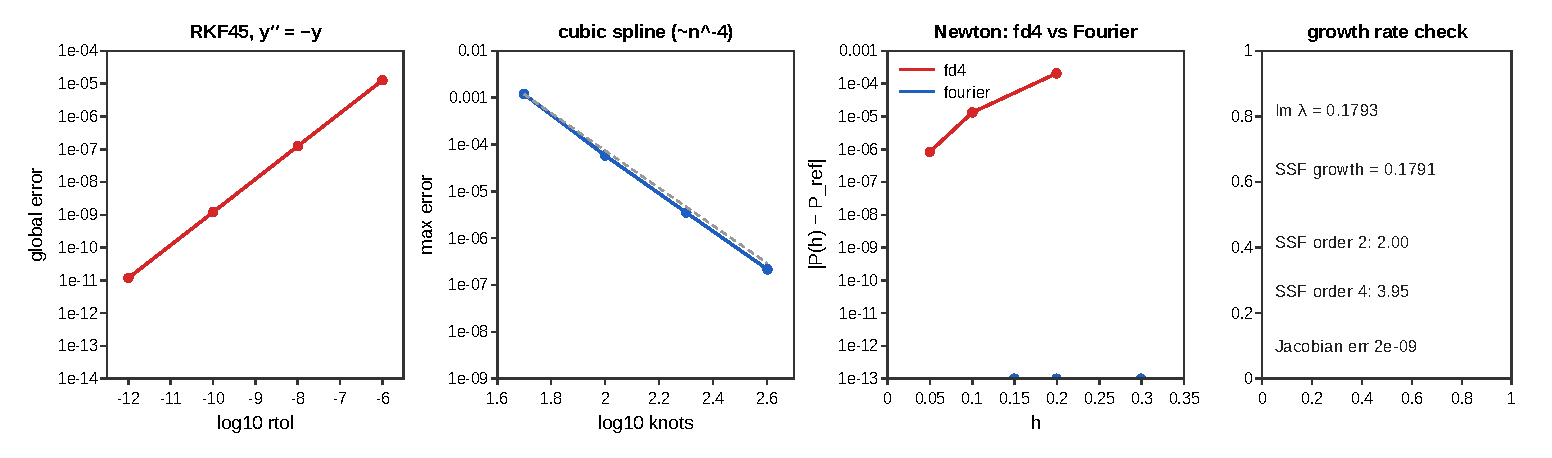
\includegraphics[width=\textwidth]{figures/fig_validation}
\caption{\label{fig:validation}Convergence of the building blocks, from left to right: RKF4(5)
error against tolerance; cubic-spline error against the number of knots ($\propto n^{-4}$);
Newton solutions with fourth-order differences against the Fourier discretization; eigenvalue
growth rate against the growth measured in propagation.}
\end{figure*}

\begin{figure*}[t]
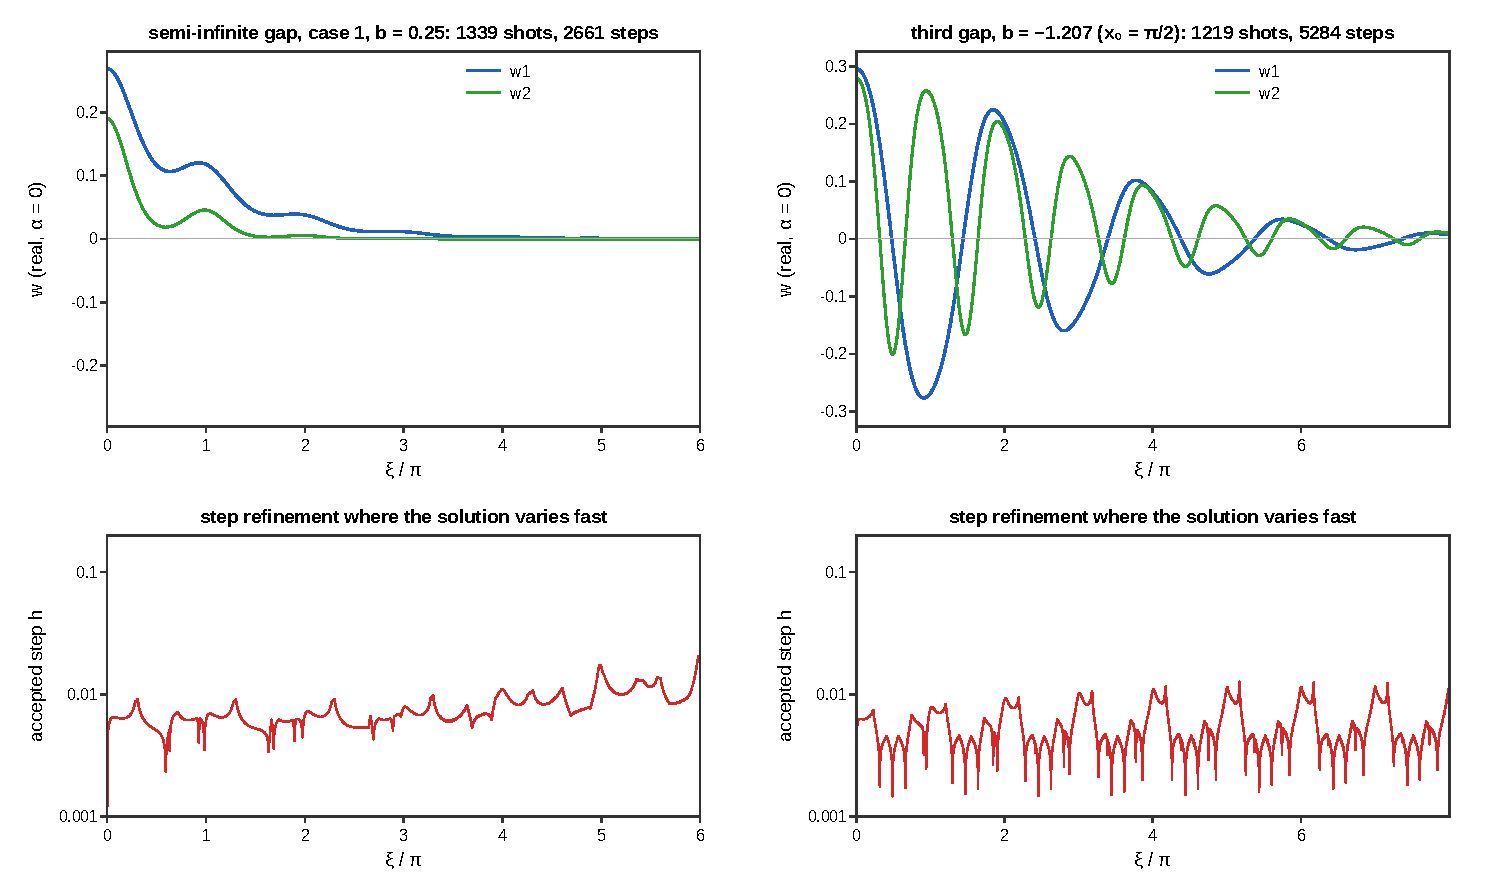
\includegraphics[width=0.85\textwidth]{figures/fig_shooting}
\caption{\label{fig:shooting}Converged edge shots at $\alpha=0$, integrated inward from
$\xi_f$ (right) to $0$, for the semi-infinite gap (case 1, $b=0.25$) and the third finite gap
($b=-1.207$, centred at $\xi_0=\pi/2$). Lower panels: accepted step size of the adaptive
integrator, which refines where the solution varies fast and coarsens in the tails.}
\end{figure*}

% =============================================================================================
\section{Results}\label{sec:results}
All results are for $V_1=V_2=1$.

\subsection{Band structure}
The SH top band edge is $b_{2+}^{(0)}=0.378489$, equal to $-a_0(2)/4$ of the Mathieu equation. At
$\alpha=0.7$ the mismatch that matches the FF and SH edges is $q_+^{(0,0)}=-0.31560$. In the third
finite gap the FF edge reaches the SH edge, $-1.29317$, at $\alpha=0.7919$ (FF edge $-1.29322$),
in agreement with Ref.~\cite{MKM2013} up to the sign convention (Fig.~\ref{fig:bands}).

\begin{figure*}[t]
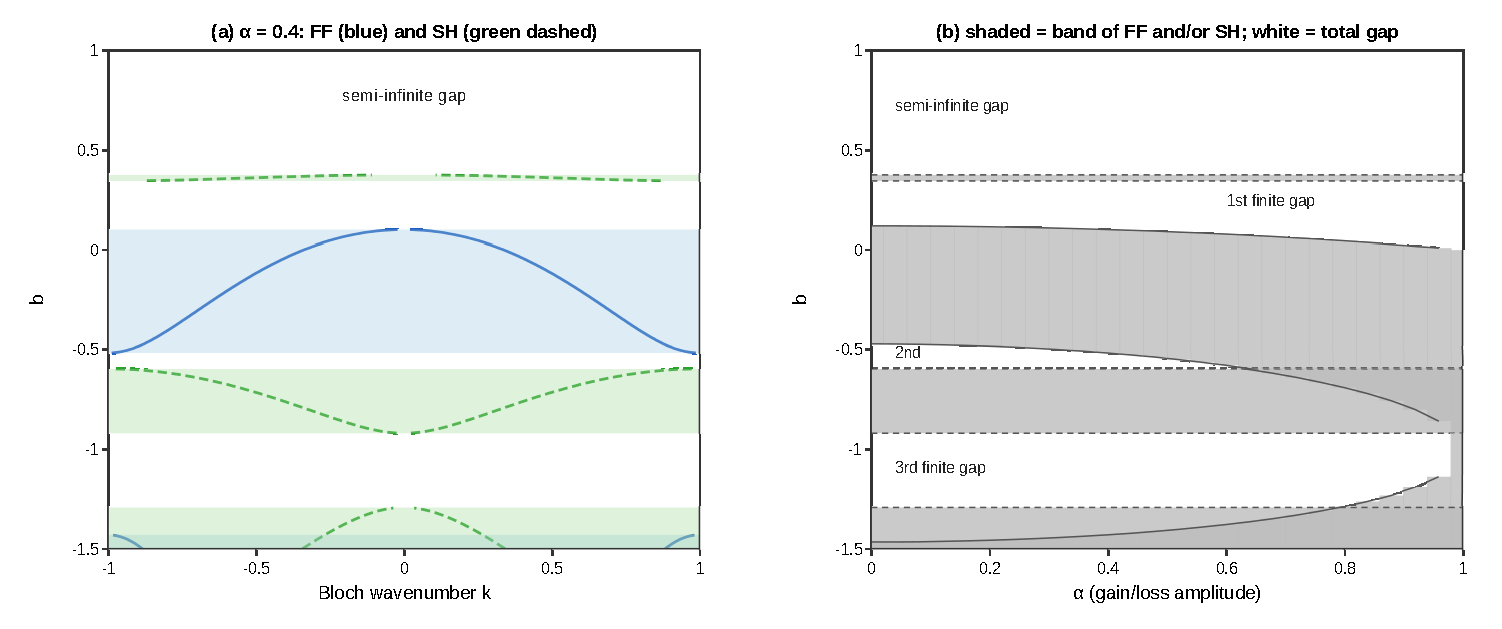
\includegraphics[width=0.9\textwidth]{figures/fig1_bands}
\caption{\label{fig:bands}Band-gap spectrum from the Floquet discriminants, $q=0$.
(a) Dispersion at $\alpha=0.4$, FF (solid) and SH (dashed).
(b) Bands against $\alpha$; shaded: band of the FF and/or SH; white: total gap. The third finite
gap closes where the FF edge meets the SH edge, $b=-1.293$, $\alpha=0.7919$.
Cf.\ Fig.~1 of Ref.~\cite{MKM2013}.}
\end{figure*}

\subsection{Semi-infinite gap}\label{sec:semiinf}
As in Ref.~\cite{MKM2013}, three cases at $\alpha=0.7$ are considered: case 1 with
$q=q_+^{(0,0)}$, case 2 with $q=0$, and case 3 with $q=-0.5134$. The families and their growth
rates are shown in Fig.~\ref{fig:semiinf}, and the profiles in Fig.~\ref{fig:semiprof}. The
examples quoted as $P=0.5$ in Ref.~\cite{MKM2013} give $P=0.4992$ (case 2, $b=0.43$) and $P=0.4970$
(case 3, $b=0.21$). In case 1 we find $P=0.388$ at the quoted $b=0.25$; the dot in the original
figure is drawn at $b\approx0.27$, where we find $P=0.444$.

\paragraph*{Stability.}
Case 1 is stable from the band edge to $b\approx0.35$ and has an internal-mode instability for
$0.35\lesssim b\lesssim0.73$. At $b=0.5$, for instance, $\lambda = \pm1.748 + 0.179i$, and
propagation gives the growth rate $0.1791$ (Fig.~\ref{fig:dyn1}). Case 2 is unstable for
$0.38\le b\le0.39$ and $0.65\le b\le0.97$, against $0.62$--$0.97$ plus a sliver at the SH edge in
the original. Case 3 is unstable for $0.20\le b\le0.53$ and $0.76\le b\le0.87$, against
$\approx0.22$--$0.58$ and $0.76$--$0.9$ in the original.

At $b=0.21$ the case-3 soliton has a weak instability, $\Img\lambda = 3.56\times10^{-3}$, at the
lower end of the first window. It is converged in the box size and confirmed by seeded propagation
($3.39\times10^{-3}$). Over $\zeta=1000$ the amplification is only $e^{3.6}$, which explains why
noisy runs of that length look stable (Fig.~\ref{fig:dyn3}).

\paragraph*{High-frequency growth.}
Inside the windows where the internal-mode instability switches off (case 1, $b\gtrsim0.73$;
case 3, $0.53\lesssim b\lesssim0.76$), a mode with $\Rea\lambda\approx\pm4.7$--$4.8$ and growth
$0.02$--$0.06$ remains. Its rate \emph{increases} with the box: in case 3 at $b=0.65$ it is
$0.050$ at $L=16\pi$ and $0.059$ at $L=24\pi$, and propagation in the $24\pi$ box gives $0.055$.
It is therefore either a convective amplification of radiation by the gain or a finite-box
effect; we do not count it as an instability of the soliton. This point needs a dedicated study
(PLAN.md, item C4).

\begin{figure*}[t]
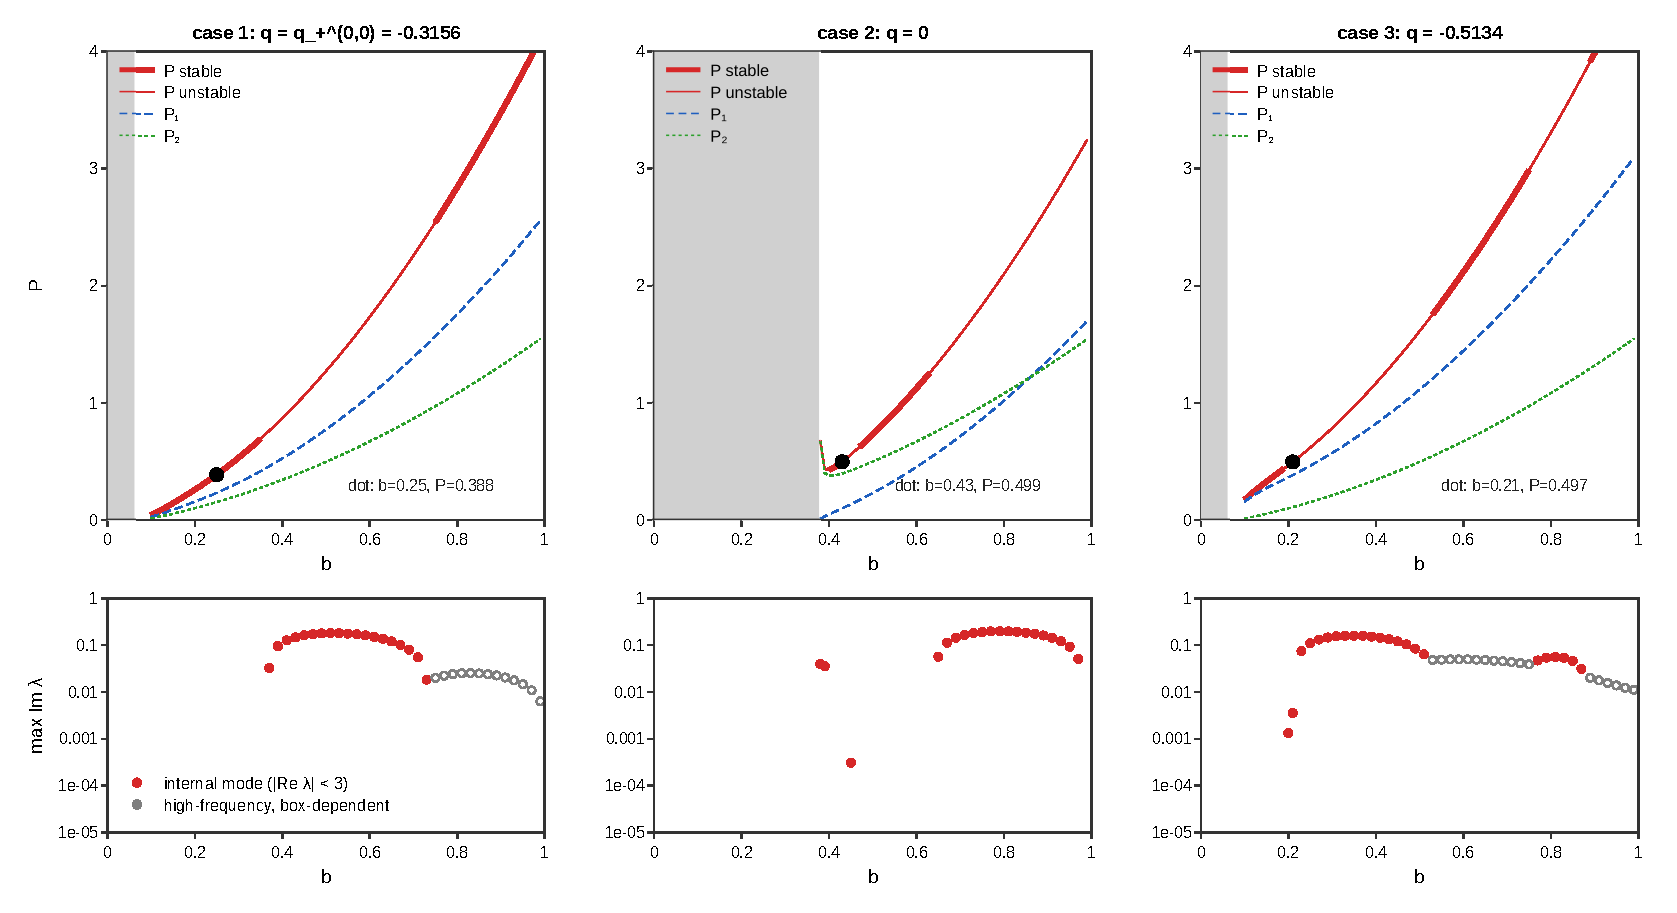
\includegraphics[width=\textwidth]{figures/fig3_semiinf_branches}
\caption{\label{fig:semiinf}Semi-infinite gap, $\alpha=0.7$: power against $b$ for cases 1--3
(thick: no internal-mode instability; thin: unstable; grey: band) and, below, the growth rate
$\max\Img\lambda$ along each family. Filled markers: internal modes ($|\Rea\lambda|<3$); open
markers: high-frequency, box-dependent growth. Cf.\ Figs.~3 and 10 of Ref.~\cite{MKM2013}.}
\end{figure*}

\begin{figure*}[t]
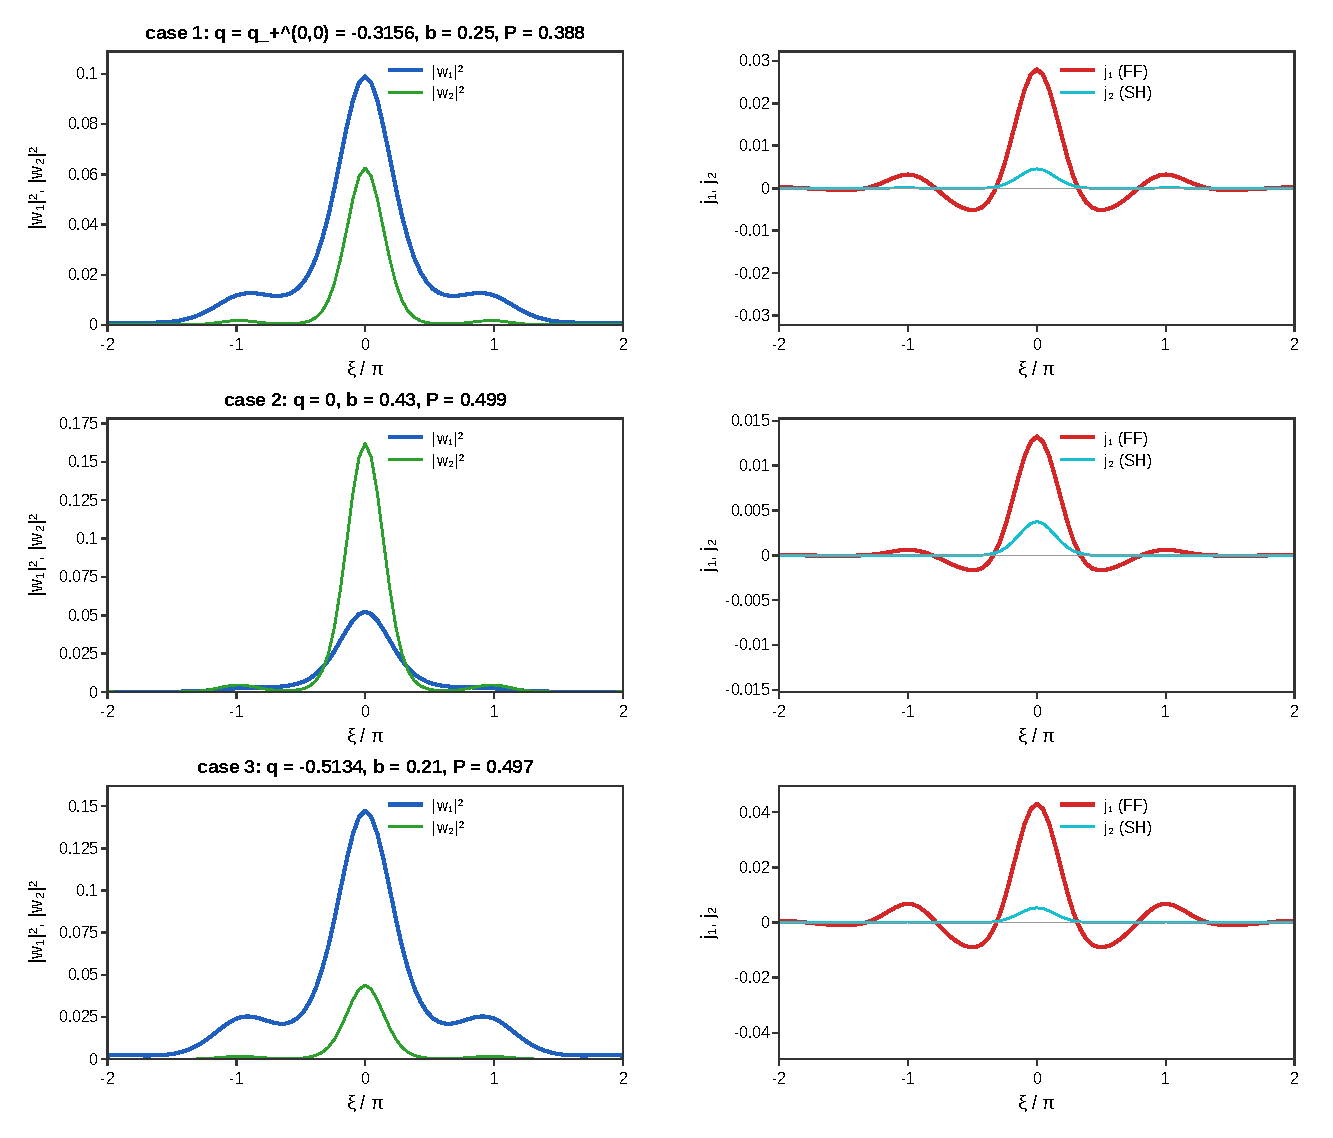
\includegraphics[width=0.8\textwidth]{figures/fig4_semiinf_profiles}
\caption{\label{fig:semiprof}Semi-infinite gap profiles $|w_l|^2$ and currents
$j_l=\Img(w_l^{*}w_l')$ for the three cases at the example points. The sign of the currents is
opposite to Ref.~\cite{MKM2013} because of the mirrored convention (Sec.~\ref{sec:model}).}
\end{figure*}

\begin{figure*}[t]
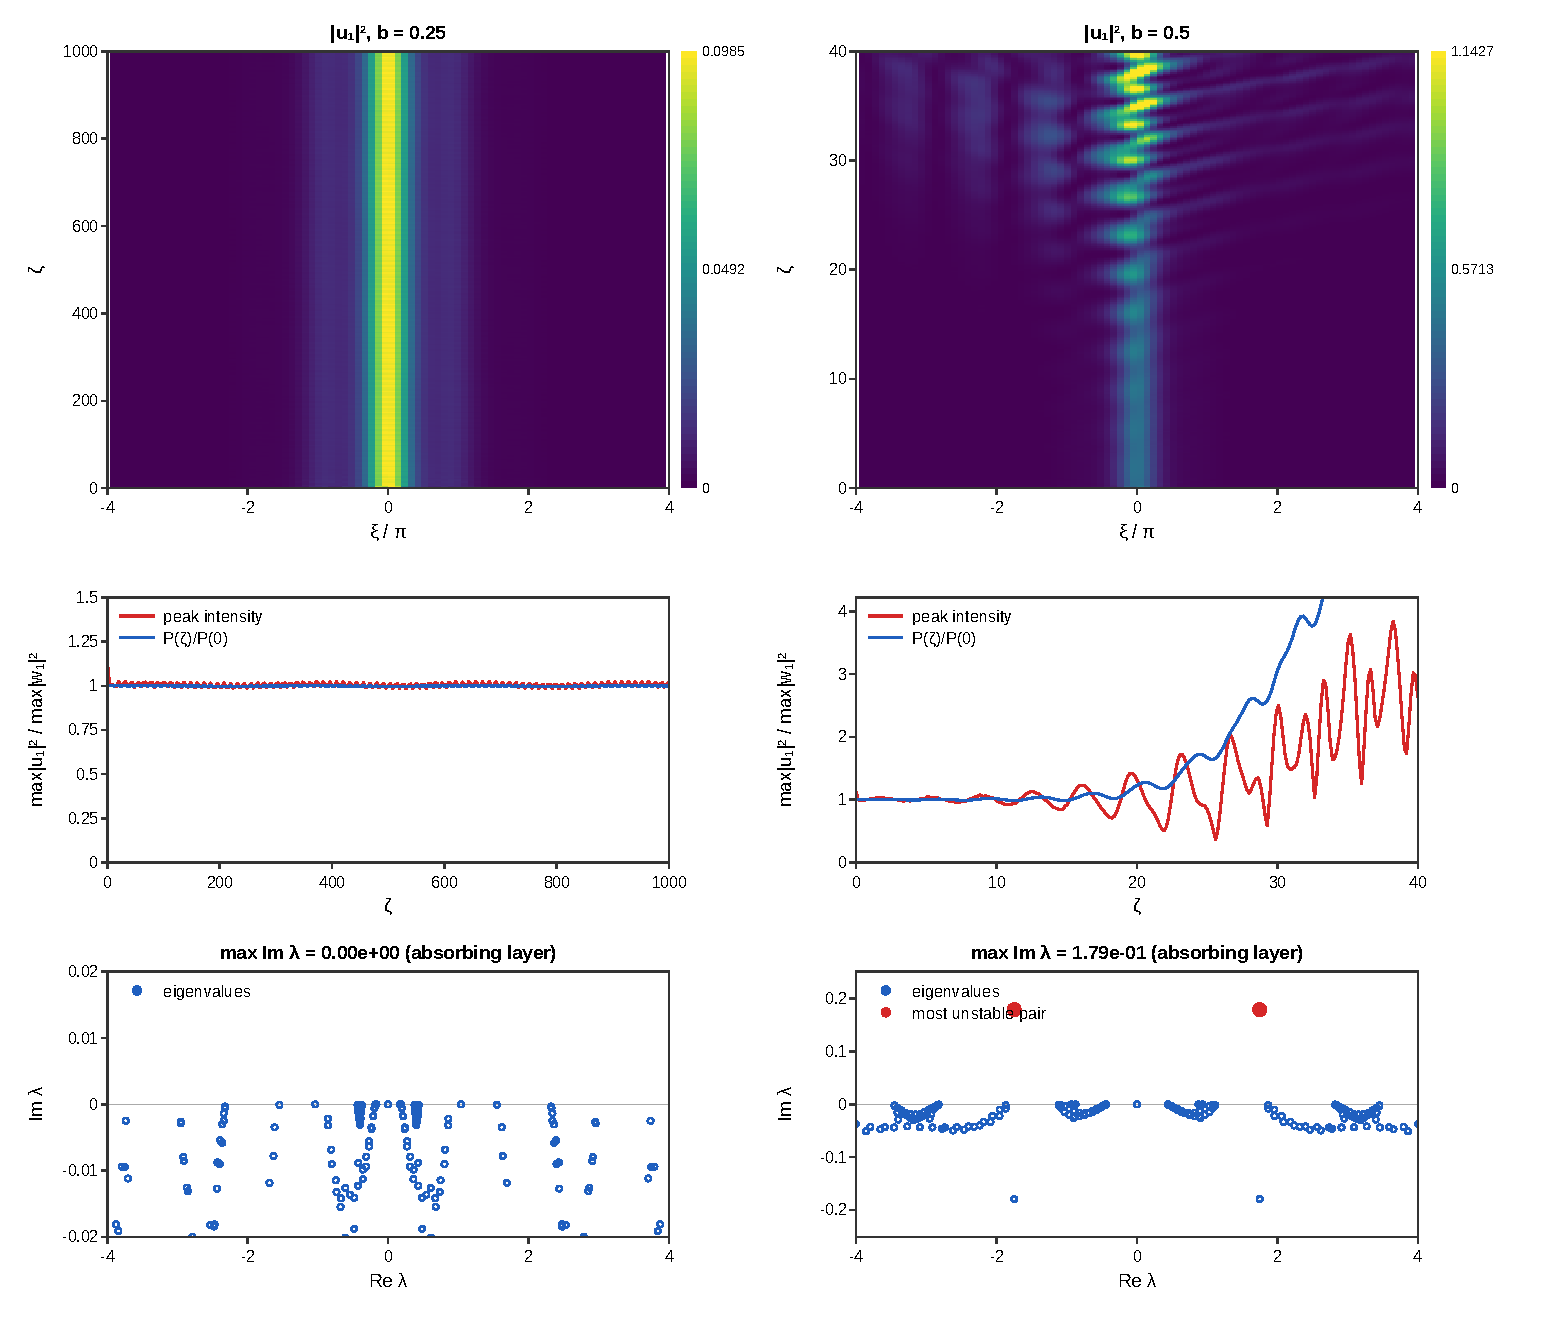
\includegraphics[width=0.85\textwidth]{figures/fig7_case1_dynamics}
\caption{\label{fig:dyn1}Case 1, $\alpha=0.7$: split-step propagation with 10\% noise and the
linear spectrum, at $b=0.25$ (left, stable; $P$ changes from $0.3901$ to $0.3898$ over $\zeta=1000$)
and $b=0.5$ (right, unstable pair $\lambda=\pm1.748+0.179i$). Rows: $|u_1|^2$, peak intensity and
$P(\zeta)/P(0)$, eigenvalues with the absorbing layer. Cf.\ Fig.~7 of Ref.~\cite{MKM2013}.}
\end{figure*}

\begin{figure*}[t]
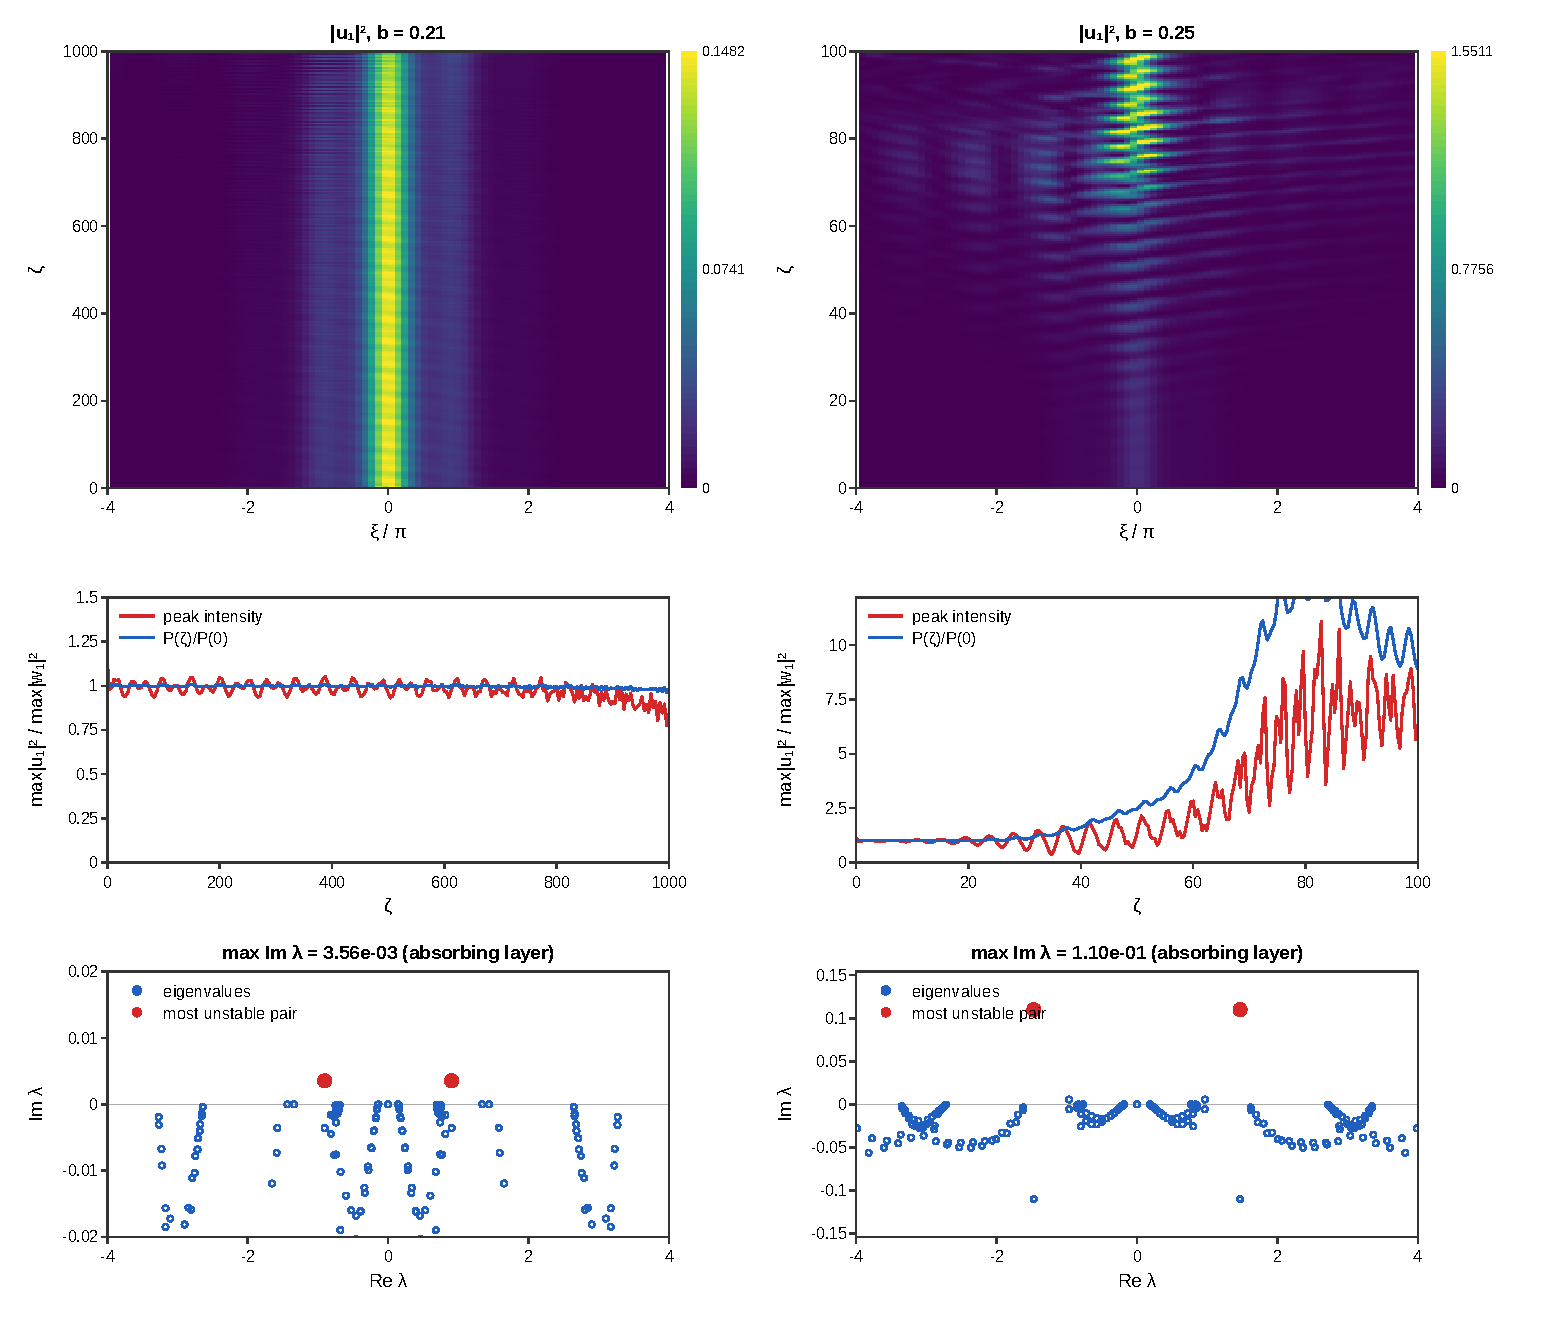
\includegraphics[width=0.85\textwidth]{figures/fig18_case3_dynamics}
\caption{\label{fig:dyn3}Case 3, $\alpha=0.7$: as Fig.~\ref{fig:dyn1} at $b=0.21$ (weakly unstable,
$\Img\lambda=3.56\times10^{-3}$) and $b=0.25$ ($\Img\lambda=0.110$). Cf.\ Fig.~18 of
Ref.~\cite{MKM2013}.}
\end{figure*}

\subsection{Third finite gap}\label{sec:thirdgap}
\paragraph*{Centring.}
At $\alpha=0$, the FF Bloch mode at the edge of this gap is odd about $\xi=0$ and even about
$\xi=\pi/2$. The fundamental gap soliton bifurcating from it is therefore centred at the lattice
minimum, $\xi_0=\pi/2$. Shooting centred at $\xi=0$ finds only multi-hump states of high
power ($P\approx15.6$ at $b=-1.207$).

\paragraph*{Families.}
With $\xi_0=\pi/2$, the shot at $b=-1.207$ gives $P=0.50097$ at $\alpha=0.7919$, the example of
Ref.~\cite{MKM2013} with $P=0.5$. The other two examples give $P=0.50242$ ($\alpha=0.7$,
$b=-1.234$) and $P=0.52329$ ($\alpha=0.9$, $b=-1.153$). The families were traced in a box $L=40\pi$, $h=0.25$ (Fourier). They reach from close to the band edge to $b\approx-1.05$ (Fig.~\ref{fig:gap3}, Table~\ref{tab:gap3}); profiles are shown in
Fig.~\ref{fig:gap3prof}.

\paragraph*{Stability of the conservative family.}
Figure~5 of Ref.~\cite{MKM2013} draws the $\alpha=0$ family as stable. We find an oscillatory
instability at every computed point, $-1.282\le b\le-1.077$, with growth rate $0.006$--$0.087$.
At $b=-1.197$ the most unstable eigenvalues are $\lambda = \pm1.540 + 0.0282i$. The rate is the
same to three digits for absorber strengths $g_0=1$ and $0.25$ and for $h=0.25$ and $0.2$
(Table~\ref{tab:conv}), and direct propagation from a $10^{-4}$ perturbation grows at $0.028$. The unstable eigenvector keeps an oscillating, slowly decaying tail. This is consistent with an
internal mode resonating with a branch of the continuous spectrum of opposite Krein signature,
which in a finite gap can lie at the frequency of the internal mode. This is the known mechanism
of oscillatory instabilities of gap solitons \cite{Barashenkov1998,Pelinovsky2004}. \todo{Krein-signature computation to confirm the
mechanism (PLAN.md, C3).}

\paragraph*{$\PT$ families.}
The oscillatory mode of the conservative family persists for $\alpha>0$, with
$\Rea\lambda\approx1.2$--$1.4$, but the gain--loss weakens it strongly. At $b=-1.207$ its rate is
$0.026$ for $\alpha=0$, $4.0\times10^{-3}$ for $\alpha=0.7$ and $1.0\times10^{-3}$ for
$\alpha=0.7919$; at $b=-1.137$ it is $0.046$, $0.013$ and $6.0\times10^{-3}$
(Fig.~\ref{fig:gap3}, right). At $\alpha=0.7919$ and $b=-1.207$ the mode sits at
$\Rea\lambda=\pm1.298$, and seeded propagation gives the rate $1.07\times10^{-3}$. Over $\zeta=1000$ the
power of a noisy run changes only from $0.5032$ to $0.5045$ (Fig.~\ref{fig:gap3dyn}). At
Deeper in the gap a purely imaginary eigenvalue with rate $0.1$--$0.3$ takes over: for
$b\gtrsim-1.12$ at $\alpha=0.7$ and $0.7919$, $b\gtrsim-1.105$ at $\alpha=0.9$, and
$b\gtrsim-1.09$ at $\alpha=0.95$. At $b=-1.101$, Ref.~\cite{MKM2013} reports a purely imaginary pair
and decay. We also find a purely imaginary eigenvalue, $\lambda=0.201i$, but the propagated soliton
\emph{grows} rather than decays: driven by the gain, $P$ goes from $2.09$ to $750$ by $\zeta=100$.

Close to the band edge, the most unstable eigenvalue of every $\alpha>0$ family in the production box
is purely imaginary, with rate $3\times10^{-5}$--$6\times10^{-4}$. The rate \emph{increases}
toward the edge as the soliton broadens and its tails reach the absorbing layer. Section~\ref{sec:conv}
shows that these rates fall by factors of 6 to 18 when the box grows from $40\pi$ to $56\pi$. They
are therefore box artefacts, and these parts of the families are stable within our resolution, as
drawn in Ref.~\cite{MKM2013}. In Fig.~\ref{fig:gap3} and Table~\ref{tab:gap3}, weak purely
imaginary modes ($|\Rea\lambda|<0.05$, $\Img\lambda<10^{-3}$) are accordingly classified as
box-dependent and not counted as instabilities. This rule changes nothing in the semi-infinite gap,
where all such modes are below $2\times10^{-5}$.

\begin{table*}[t]
\caption{\label{tab:gap3}Third-gap families ($q=0$, $\xi_0=\pi/2$, $L=40\pi$, $h=0.25$): band edge,
traced range of $b$, power range, number of unstable points among those with a computed spectrum,
and range of the growth rate. Internal modes only: $|\Rea\lambda|<3$, $\Img\lambda>5\times10^{-5}$,
and weak purely imaginary near-edge modes excluded (Sec.~\ref{sec:conv}) (results/thirdgap.json).}
\footnotesize
% generated by make_tables.py from results/thirdgap.json -- do not edit
\begin{tabular}{cccccc}
\hline\hline
$\alpha$ & edge $b_{\rm e}$ & traced $b$ & $P$ & unstable points & $\max\mathrm{Im}\,\lambda$\\
\hline
0.0 & $-1.2932$ & $[-1.287,\,-1.067]$ & $0.843$--$4.39$ & 16/16 & $6.1\times10^{-3}$--$0.087$\\
0.7 & $-1.2932$ & $[-1.287,\,-1.067]$ & $0.116$--$5.37$ & 15/16 & $1.1\times10^{-4}$--$0.314$\\
0.7919 & $-1.2932$ & $[-1.272,\,-1.067]$ & $0.058$--$3.90$ & 12/15 & $9.7\times10^{-5}$--$0.291$\\
0.9 & $-1.2118$ & $[-1.185,\,-1.060]$ & $0.242$--$2.53$ & 9/12 & $1.1\times10^{-4}$--$0.235$\\
0.95 & $-1.1530$ & $[-1.110,\,-1.040]$ & $0.521$--$2.54$ & 3/5 & $6.2\times10^{-2}$--$0.214$\\
\hline\hline
\end{tabular}

\end{table*}

\begin{figure*}[t]
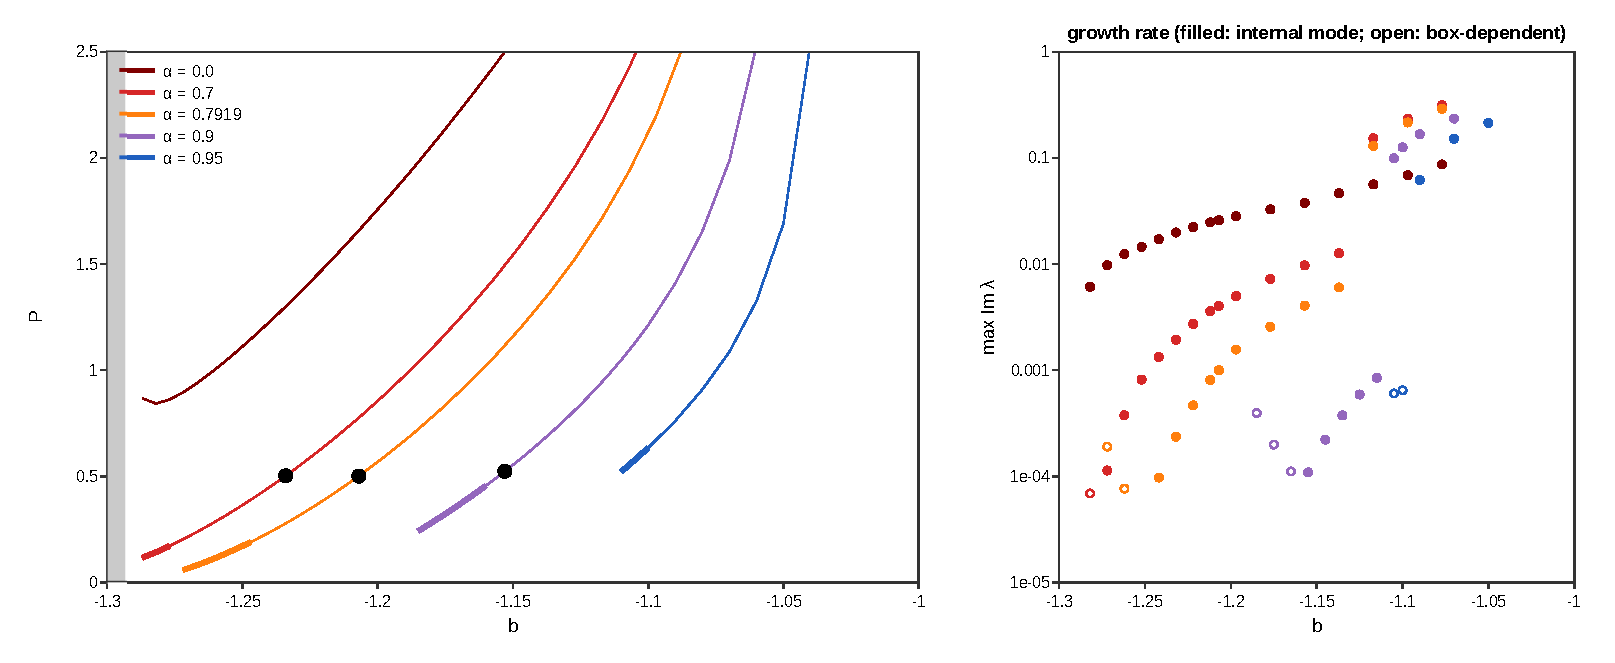
\includegraphics[width=\textwidth]{figures/fig5_thirdgap_branches}
\caption{\label{fig:gap3}Third finite gap, $q=0$, solitons centred at $\xi_0=\pi/2$. Left: power
against $b$ for $\alpha=0$, $0.7$, $0.7919$, $0.9$, $0.95$ (thick: linearly stable; thin:
unstable; grey: SH band). Dots: the examples of Fig.~\ref{fig:gap3prof}. Right: growth rate along
each family; filled: internal modes; open: box-dependent (weak purely imaginary near-edge modes,
Sec.~\ref{sec:conv}). Cf.\ Fig.~5 of Ref.~\cite{MKM2013}.}
\end{figure*}

\begin{figure*}[t]
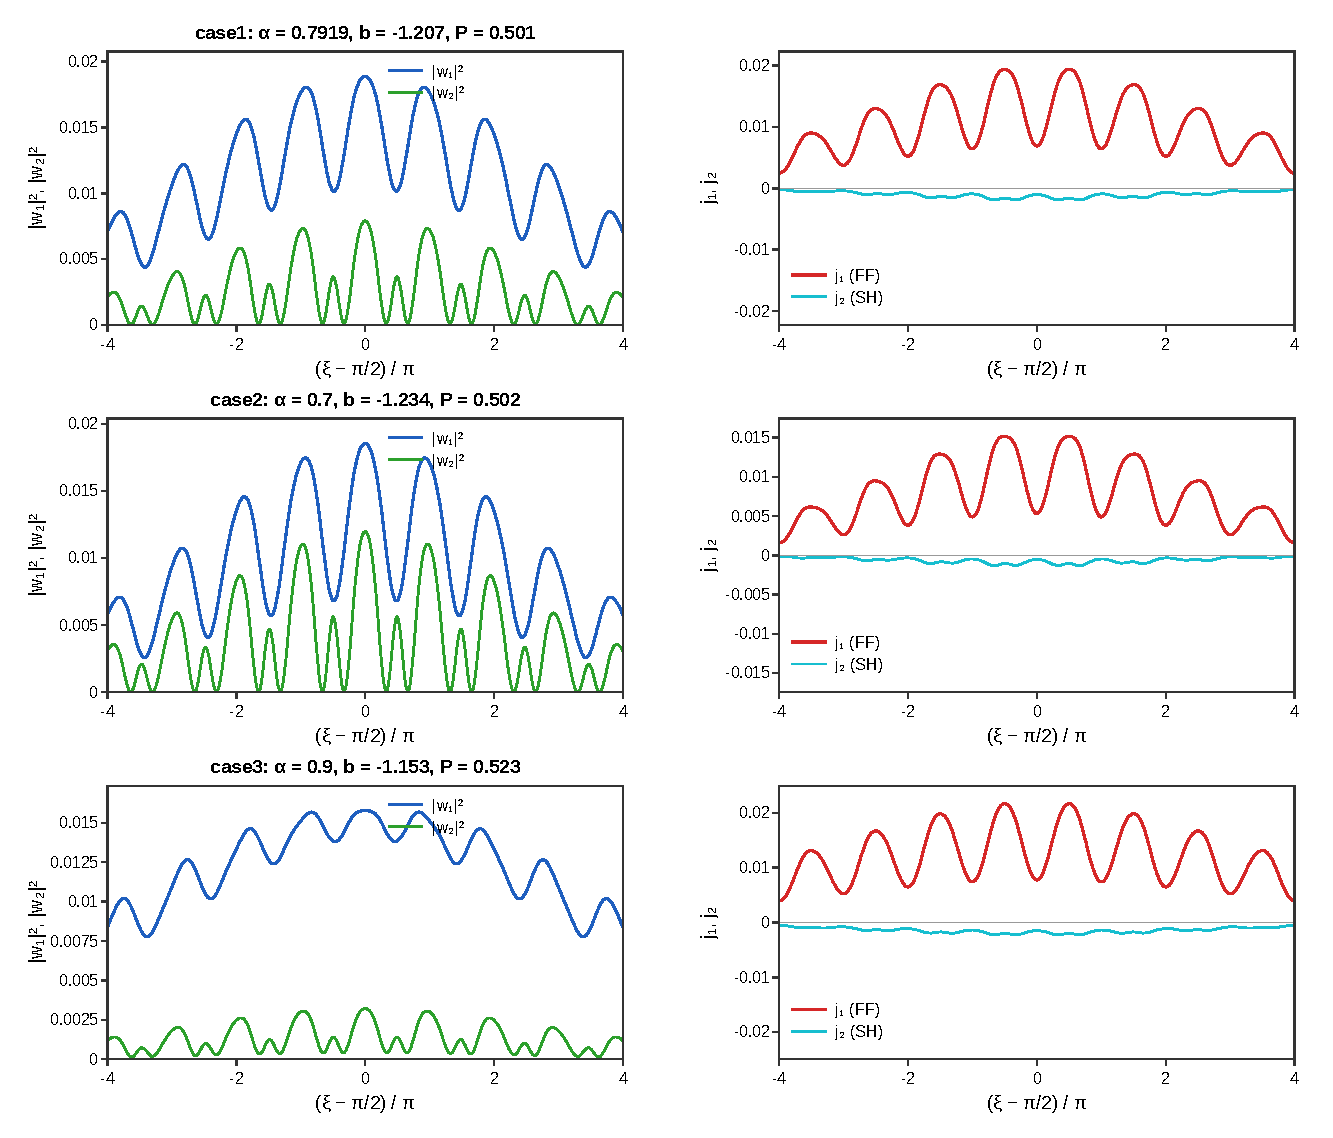
\includegraphics[width=0.8\textwidth]{figures/fig6_thirdgap_profiles}
\caption{\label{fig:gap3prof}Third-gap profiles and currents:
$\alpha=0.7919$, $b=-1.207$ ($P=0.501$);
$\alpha=0.7$, $b=-1.234$ ($P=0.502$);
$\alpha=0.9$, $b=-1.153$ ($P=0.523$).
Cf.\ Fig.~6 of Ref.~\cite{MKM2013}.}
\end{figure*}

\begin{figure*}[t]
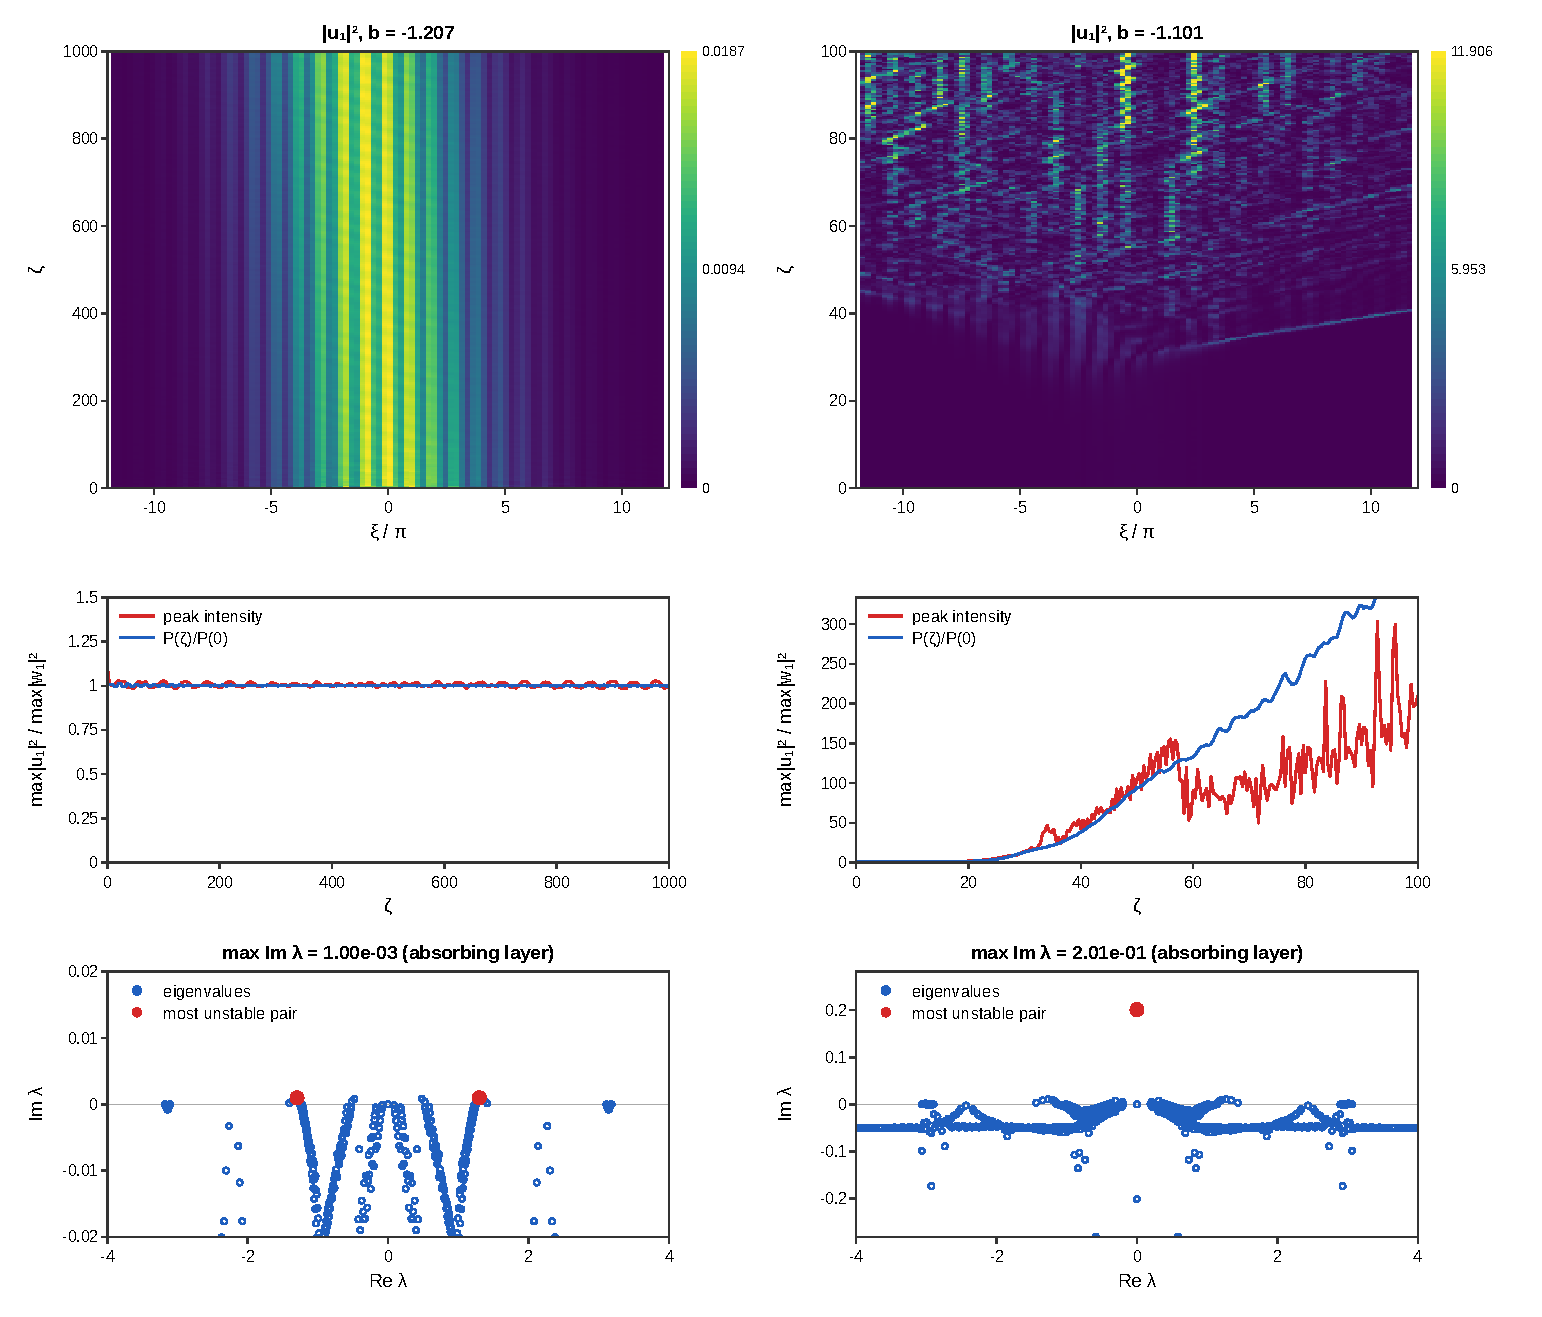
\includegraphics[width=0.85\textwidth]{figures/fig8_thirdgap_dynamics}
\caption{\label{fig:gap3dyn}Third finite gap, $\alpha=0.7919$: propagation with 10\% noise and the
linear spectrum at $b=-1.207$ (left; $\Img\lambda=1.0\times10^{-3}$, $P$ changes from $0.5032$ to
$0.5045$ over $\zeta=1000$) and $b=-1.101$ (right; $\lambda=0.201i$, gain-driven growth). Cf.\ Fig.~8
of Ref.~\cite{MKM2013}.}
\end{figure*}

\subsection{Convergence of the third-gap growth rates}\label{sec:conv}
Table~\ref{tab:conv} gives the growth rate at selected points for three grids: the production
grid, a finer step, and a larger box. Each grid is shown for two absorber strengths.

The oscillatory instabilities are converged. For $\alpha=0$ at $b=-1.197$ the rate is $0.0282$ on
all three grids and for both absorbers. For $\alpha=0.7919$ at $b=-1.207$ it is
$(1.0\pm0.1)\times10^{-3}$. Refining $h$ from $0.25$ to $0.2$ changes no rate in the first three
digits, so the Fourier grid resolves the eigenvectors. Near the band edge, at $\alpha=0$ and
$b=-1.282$, the soliton is wide and the rate with the weaker absorber is not yet converged at
$L=40\pi$: $1.03\times10^{-2}$ against $6.10\times10^{-3}$. At $L=56\pi$ the two values close in,
to $7.03\times10^{-3}$ and $6.15\times10^{-3}$. The instability is real, with a rate of about
$6\times10^{-3}$.

The purely imaginary near-edge modes behave differently. At $\alpha=0.7$, $b=-1.282$ the rate
drops from $6.9\times10^{-5}$ to $1.2\times10^{-5}$, and the most unstable eigenvalue becomes the
oscillatory mode ($|\Rea\lambda|=1.39$). At $\alpha=0.7919$, $b=-1.262$ the rate drops from
$7.7\times10^{-5}$ to $4.3\times10^{-6}$. A rate that decreases with the box is a property of the
box, not of the soliton. The near-edge points of the $\alpha=0.9$ and $0.95$ families
($\Img\lambda$ up to $6\times10^{-4}$) were not tested on the larger box
\todo{PLAN.md, C2}.

\begin{table*}[t]
\caption{\label{tab:conv}Growth rate $\max\Img\lambda$ at selected third-gap points for three grids
(Fourier differentiation), with absorbing layer $g_0=1$ and, in parentheses, $g_0=0.25$. Last
column: $|\Rea\lambda|$ of the most unstable eigenvalue on the largest box (results/convergence.json).}
\footnotesize
% generated by make_tables.py from results/convergence.json -- do not edit
\begin{tabular}{cccccc}
\hline\hline
$\alpha$ & $b$ & $L=40\pi$, $h=0.25$ & $L=40\pi$, $h=0.2$ & $L=56\pi$, $h=0.25$ & $|\mathrm{Re}\,\lambda|$\\
\hline
0.0 & $-1.197$ & $2.82\times10^{-2}$ ($2.81\times10^{-2}$) & $2.82\times10^{-2}$ ($2.81\times10^{-2}$) & $2.82\times10^{-2}$ ($2.82\times10^{-2}$) & $1.540$\\
0.0 & $-1.282$ & $6.10\times10^{-3}$ ($1.03\times10^{-2}$) & $6.10\times10^{-3}$ ($1.03\times10^{-2}$) & $6.15\times10^{-3}$ ($7.03\times10^{-3}$) & $1.444$\\
0.7 & $-1.282$ & $6.89\times10^{-5}$ ($5.62\times10^{-5}$) & $6.89\times10^{-5}$ ($5.62\times10^{-5}$) & $1.17\times10^{-5}$ ($1.12\times10^{-5}$) & $1.386$\\
0.7919 & $-1.262$ & $7.66\times10^{-5}$ ($6.18\times10^{-5}$) & $7.66\times10^{-5}$ ($6.18\times10^{-5}$) & $4.25\times10^{-6}$ ($3.16\times10^{-6}$) & $0.000$\\
0.7919 & $-1.207$ & $1.00\times10^{-3}$ ($9.80\times10^{-4}$) & $1.00\times10^{-3}$ ($9.80\times10^{-4}$) & $9.92\times10^{-4}$ ($1.12\times10^{-3}$) & $1.298$\\
\hline\hline
\end{tabular}

\end{table*}

% =============================================================================================
\section{Summary of differences with Ref.~\cite{MKM2013}}
\begin{enumerate}
\item \emph{Sign convention.} The figures correspond to the printed stationary equations with
$b\to-b$. Equations (9) and (10) of Ref.~\cite{MKM2013} give the mismatch $q$ with opposite signs,
and the numbers follow Eq.~(10). The third-gap matching value printed as $1.29$ is $-1.29$.
\item \emph{Centring.} The fundamental third-gap soliton sits at the lattice minimum.
\item \emph{Third gap, $\alpha=0$.} The family is oscillatorily unstable. For $\alpha>0$ the same
mode persists with a rate reduced by one to two orders of magnitude.
\item \emph{Weak instabilities.} Rates of order $10^{-3}$, confirmed by propagation, occur at
points drawn as stable: case 3 at $b=0.21$, and the third gap at $\alpha=0.7919$, $b=-1.207$.
\item \emph{Third gap, $\alpha=0.7919$, $b=-1.101$.} The unstable soliton grows under the gain
rather than decaying.
\item \emph{Agreements.} The instability windows of cases 2 and 3 agree with Fig.~10 of
Ref.~\cite{MKM2013} to within $\delta b\approx0.03$--$0.05$. Near the band edge, the $\alpha>0$
third-gap families are stable within resolution, as drawn there.
\end{enumerate}

\section{Conclusions}
An independent, fully validated implementation of the numerical methods for $\chit$ gap solitons
in $\PT$-symmetric lattices reproduces the existence results of Ref.~\cite{MKM2013} quantitatively.
It also exposes a sign convention, the centring of third-gap solitons, and instabilities that the
original analysis missed or could not resolve, the largest being the oscillatory instability of
the conservative third-gap family. Three numerical ingredients were decisive: the forced Floquet
tail in the shooting, the $\PT$-symmetric half-domain Newton solver, and the absorbing layer in
the stability problem. The open question is the high-frequency growth found in the stability windows: whether it is a
property of the infinite system or a finite-box effect.

\appendix
% =============================================================================================
\section{Forced Floquet tail}\label{app:tail}
Let $\phi_1$ be the decaying FF Floquet solution, normalized at $\xi_f$. The SH equation in the
tail, $\psi'' = -Q_2\psi - 2\phi_1^2$, has a particular solution with $\psi(\xi+\pi) = \mu_1^2\psi(\xi)$.
Write $\bm y=(\psi,\psi')^{\mathsf T}$. Integrating over one period gives
$\bm y(\pi) = M_2\bm y(0) + \bm g$, where $\bm g$ is the solution at $\pi$ of the forced equation
with zero initial data. Requiring $\bm y(\pi) = \mu_1^2\bm y(0)$ gives Eq.~(\ref{eq:forced}). This
solution exists when $\mu_1^2$ is not a multiplier of the SH operator, which holds in a total gap.

\section{Linear stability operator}\label{app:stab}
Insert $u_1 = e^{ib\zeta}(w_1+p_1)$ and $u_2 = e^{2ib\zeta}(w_2+p_2)$ into
Eqs.~(\ref{eq:u1})--(\ref{eq:u2}) and linearize:
\begin{align*}
i\partial_\zeta p_1 &= -\mathcal M_1p_1 - 2w_1^{*}p_2 - 2w_2p_1^{*},\\
i\partial_\zeta p_2 &= -\mathcal M_2p_2 - 2w_1p_1.
\end{align*}
Then substitute $p_1 = ae^{-i\lambda\zeta}+c^{*}e^{i\lambda^{*}\zeta}$ and
$p_2 = de^{-i\lambda\zeta}+f^{*}e^{i\lambda^{*}\zeta}$. Collect the $e^{-i\lambda\zeta}$ terms, and
the complex conjugate of the $e^{i\lambda^{*}\zeta}$ terms. This gives Eq.~(\ref{eq:stab}); note
that $\mathcal M_2$ is real.

% =============================================================================================
\section*{Data and code availability}
All code (Python/NumPy), the computed data (results/*.json) and the scripts that produce every
figure and table are in the repository
\url{https://github.com/hypervanse/Saturable-nonlinearity-non-PT} (folder pt\_chi2\_periodic).
\todo{archive with a DOI, e.g.\ Zenodo, before submission}

\begin{acknowledgments}
\todo{funding and acknowledgments.}
\ifaiauthor\else
\emph{Use of AI.} The numerical code, the computations, the figures and a first draft of this
manuscript were produced by the AI system Claude Opus 5.5 (Anthropic) working in Claude Code,
following the algorithms of Ref.~\cite{MoreiraThesis} and under the direction of F.~C.~Moreira,
who reviewed all results and is responsible for the content.
\fi
\end{acknowledgments}

\bibliography{refs}

\end{document}
